\chapter{Tracing Optimizations}\label{ch:5}
Read/write tracing is used to correctly emulate self-referential and self-modifying code in the guest, and to steal guest data address space for the translation cache. Tracing results in extra page faults, and these page faults can result in significant performance degradation. In fact, without any optimizations, the number of such page faults is far greater than the number of exits caused due to privileged instructions in unmodified KVM running a Linux guest.
We implement two optimizations to reduce tracing page faults. Our first optimization adaptively resizes the guest’s pages to reduce false sharing. Our second optimization adaptively mirrors guest data (which is causing a large number of faults) to reduce the number of page faults caused by read accesses (which is the common case). For the second optimization we also translate the faulting instruction to access the mirrored data. We discuss both optimizations in detail below.

\section{Adaptive Page Resizing}
Typical TLB sizes on embedded Power Architecture processors are small. For example, the software-managed TLB on our test system is a combination of a 16-entry fully-associative cache of variable-sized page table entries and a 512-entry 4-way set-associative fixed-size (4KB) page table entries. A faster L1 TLB lookup cache is implemented in hardware, and all invalidations to maintain consistency with the software-programmed L2 TLB are done automatically. The variable-pagesize TLB cache supports 11 different page sizes: 4K, 16K, 64K, 256K, 1M, 4M, 16M, 64M, 256M, 1G, and 4G. Further a page of size S must be S-byte aligned in physical and virtual address spaces.

As explained in Section~\ref{memory_management} the hypervisor has full flexibility to control the shadow tlb entries for mapping the guest tlb entries. It can even map multiple shadow entries corresponding to a single guest tlb entry. To minimize TLB pressure, the hypervisor typically uses one shadow TLB entry per guest TLB entry. For example, if the guest uses 4MB pages, then the shadow TLB will also have corresponding entries for 4MB pages. Most operating systems use huge pages (using the variable pagesize TLB cache) for the kernel to reduce TLB pressure. The fixed pagesize TLB cache (containing map- pings for 4K pages) is made available primarily for user programs. For example, our Linux guest uses just one 256MB TLB entry mapping all its kernel code and data. Disabling read/write privileges from this TLB entry predictably causes an unacceptably large number of page faults (every kernel data access becomes a page fault).

Most of tracing faults are due to the false sharing as a result of the huge pages used by the OS. The problem can be avoided/reduced by resizing the shadow tlb entries into smaller entries to reduce tracing page faults due to read/write tracing. This will reduce false sharing resulting in less of the data section to be traced and a less number of tracing page faults. Also breaking a shadow tlb entry into multiple entries leads to increased tlb pressure and an increase in tlb misses again degrading the performance. Thus page resizing essentially is a tradeoff between the tracing page faults and increased tlb pressure.

We resize shadow TLB entries to deal with this overhead of page faults due to read/write tracing. While patching a guest privilege instruction, if the shadow tlb entry for the page containing this patch-site is not already traced and this patch-site is contained in a huge page, then the page (and the corresponding shadow tlb entry) containing this patch-site is fragmented into smaller entries such that the entry contining the patch-site is atmost 1MB large. Also on a traced page, if we notice a high number of tracing page faults on that page, we break the page into smaller fragments (and the corresponding TLB entry into smaller TLB entries). To minimize false sharing, we keep the size of the page containing the patch-site as small as possible, without adversely effecting performance. All other pages created by this fragmentation are sized as large as possible, to minimize the overall number of TLB entries. While smaller pages reduce false sharing, they also result in increased TLB pressure.

Breaking a large page potentially creates many smaller pages due to alignment restrictions. For example, if the kernel has mapped itself using a 256MB page at virtual address (0xc0000000,0xcfffffff), and a patch is to be applied at address 0xc0801234, and we have decided to break the patch-site page into a 4MB page, the new set of TLB entries will be for addresses (0xc0000000, 0xc03fffff); (0xc0400000, 0xc07fffff) (0xc0800000, 0xc0bfffff); (0xc0c00000, 0xc0ffffff); (0xc1000000, 0xc1ffffff); (0xc2000000, 0xc2ffffff); (0xc3000000, 0xc3ffffff); (0xc4000000, 0xc7ffffff); (0xc8000000, 0xcbffffff); (0xcc000000, 0xcfffffff). Notice that each page of size S is S-byte aligned and S is always one of the values supported by the architecture. Thus fragmentation of a single entry in this case has lead to 10 smaller shadow entries resulting in an increase in tlb pressure and tlb misses.

If a large number of tracing page faults are noticed on a page smaller than 64KB, then instead of fragmenting it further we remove all the patch-sites from this region and re-instate it's original read/write permissions. This is done in order to prevent the tlb thrashing which results due to excessive fragmentation of a tlb entry. This decision on whether to remove the patch-sites also depends on tradeoff between the number of privileged instruction exits due to privilege instructions on this page and the tracing page faults experienced at that point of guest's execution.

On noticing a large number of tracing page faults on a traced page, we fragment it into smaller pages to reduce false sharing. The fragmentation policy needs to be different for different profiles of tracing page faults. We use two different policies in our implementation depending on the nature of page faults. Typically page faults either occur in bursts (a large number of faults occur on a  small set of closely-located addresses on a single large page) or in scans (faults are spread over a large region with a small number of faults per address). for e.g if a data section get's traced due to false sharing, we generally observe bursts of accesses on such regions while examples of scan are during the self modifying behavior of the guest. 

For bursts, the ideal way to resize the pages is to detect the region in the page where the page faults are concentrated and resize the page such that the page faults belong to a single smaller tlb entry and then untrace this entry. This smaller entry should be kept as small as possible (without thrashing the tlb too much) since there is tradeoff between the privileged exits on this region and the page faults. We use a threshold of 20000 tracing page faults within 100ms to detect the need for page resizing. If these faults are concentrated in a small region then a burst has been deteced and we resize this page such that the concentrated page fualts belong to a 64KB page and trace is removed form this page and the corresponding patch-sites are removed. For scans, where the tracing page faults are distributed across a large address range, the page is broken into two halves (4 shadow tlb entries) and the half with larger number of tracing page faults is untraced. We do this only if the number of tracing page faults is greater than threshold $T$ of this page. 

Also if a region has been untraced earlier due to either a burst or scan detected on that region, it can be traced again as soon as the number of privilege exits on this region are greater than the threshold T of this page. These conversion from traced to untraced and vice-versa may lead to tlb thrashing due to continuous fragmentation of the pages. To resolve this we opportunistically merge the pages to larger pages after every periodic interval (100ms in our implementation). If we find pages with similar {\tt rwx} privileges we merge them to form a larger page (shadow entries for these pages might merge or not since the combined size of these pages might not be supported on the system). This opportunistically merging helps in reducing the tlb pressure and thus improves the performance.

The threshold $T$ is determined dynamically, as it depends on the tradeoff between the number of privileged instruction exits and tracing  page faults on that page. On tracing a page, we record the number of privileged instruction exits that this page was experiencing, before it got patched and traced. This serves as our threshold $T$ for that page. If the number of tracing page faults we are experiencing on this page is greater than $T$, we untrace it by removing all it's patches. On each tracing or untracing event on a page, the threshold $T$ is updated and is used to determine whether to again trace or untrace the page during future execution. Hence, after a page is untraced, $T$ is also used to determine whether to retrace it or not (we retrace if the number of privileged instruction exits > $T$).

Our dynamic thresholding mechanism relies on the assumption that the expected number of privileged instruction exits (or page faults) after  untracing (or after re-tracing) will be similar to what had been observed previously. If the guest has time-varying behaviour, it can result in bad decision-making and consequently performance penalties. For example, a guest may execute a privileged instruction a large number of times in the beginning and then never execute it again. This may result in T being raised to a large value in the beginning causing the page to remain traced unnecessarily, and thus resulting in tracing page faults that could have been avoided. To avoid such situations, our threshold T decreases linearly with time at the rate of 2000 per 100 ms. 

Adaptive page resizing significantly reduces the number of page faults. It uses the spatial and time locality of the privileged exits and tracing page faults to trace/untrace a region or to patch/unpatch a page. For example, a Linux guest boots in 13.03 seconds (as opposed to 30.03 seconds on unmodified KVM) with in-place binary translation and adaptive page resizing for read/write tracing. Without adaptive page resizing, the guest livelocks at boot time due to the large number of page faults. A detailed study of the performance tradeoffs is presented in Section~\ref{adaptive_pr_results}.

\section{Adaptive Data Mirroring}
\label{adaptive_dm}
Adaptive page resizing profiles the exits both thr privilege exits and tracing page faults and tries to pick the best at the cost of other. Thismechansim works well when the privilege text and data sections are far apart but fails when they are close enough and both of them are frequently used. For example the function dispatch tables and the exception handlers are located within the kernel text section and resides close (within 64KB region of it) to the privileged text accessing them. Both of them are frequently executed and accessed causing the adaptive page resizing algorithm perform bad due to increase in the tlb pressure. We can observe a 10-20\% performance overhead in Table~\ref{tab:detailed_results}. 

We avoid these faults by dynamically monitoring such tracing page faults, adaptively copying the data being accessed to the shared space between the host and the guest and translating the instructions to access them from their new location. This optimization prevents furter page faults on this data. 

We perform this optimization if the number of tracing page faults due to a certain read-access instruction exceeds a threshold (we use a threshold of 200 accessess). On noticing such faults, we copy the data being accessed to a “data cache”. This data cache is maintained in the read/write shared page also storing the guest’s emulated registers. The faulting instruction is replaced with code to check the data cache for the address being read. If the check succeeds, the translated code reads the data from the cache, thus avoiding a page fault. If the check fails, the translated code executes the original instruction just as before (which may result in a page fault just as before). If the hit rate of the data cache is high, we have reduced the number of page faults. This translation code of the fault- ing instruction is stored in the translation cache (maintained in the execute-only shared space) and the faulting instruction is replaced with a branch to this code. 
To maintain guest correctness, the pages containing patches for faulting instructions (due to tracing) need to be read/write traced too. This can potentially result in a chain-effect: tracing of these new pages can cause more tracing page faults, resulting in more pages to be patched and traced, resulting in more tracing page faults, and so on\ldots. Fortunately, we do not see this chain effect in practice. The faulting instructions that are patched typically reside on a page that is already being traced, causing this cycle to converge on the first iteration. Even if the patching of the faulting instructions requires a new read/write trace to be created, we expect this cycle to converge in 1-2 iterations. Intuitively, kernel code which causes privileged VM-exits or tracing page faults is likely to be spatially close, and will eventually lead to a small set of traced pages. We observed this behaviour in all our experiments with Linux guests. Even if the read write tracing chain becomes long, we rely on our adaptive page resizing algorithm to break this chain by removing the trace on a page (and all the associated patch-sites) if that page experiences a large number of page faults. 

Finally, we note that this optimization is also valid for write accesses. For write accesses, we translate the instruction to access the  mirrored data location directly. Other instructions trying to read/write the original data instruction trap and get emulated (or translated, if this happens frequently). All we need to make sure during the write accesses is that if the data we have mirrored is a text which can be executed, then we need to flush the contents of the data cache maintained by us at their corresponding data cache flush.

\section{Optimizing Translation Cache}
\label{tcache_optimizations}
As disscussed in Section~\ref{setup_space} stealing translation cache from data segment of the guest degrades the performance since the data sections are generally heavily accessed and every such access will result in a VM exit. For example when the initial aligned 64KB of address space is stolen from the guest {\tt RO} segment for translation cache the linux boot benchmark experiences around 1,000,000 exits due to tracing page faults which itself is pretty large number and might even increase/decrease if the space is stolen from other regions. Adaptive Data Mirroring it to data cache maintained in the shared space as discussed in the last section will also not be too effective since this region is data section and the accesses are typically widespread resulting in a large number of cache misses and thus tracing page faults. Also page resizing cannot be used to reduce page faults since we cannot remove trace from this region since this shared space needs to be traced permanently as long as binary translation optimizations are active.

In order to optimize these page faults we can mirror the original contents of the stolen space in a shared address space with the guest. This shared address space is similar to the address space used to store the emulated guest space i.e region that is not mapped/used by the guest. In other words we have increased the size of the first shared address space to be equal to the size of the stolen region for translation cache and the space used to store the emulated state of the guest. In our implementation we have used the top most region of the Linux guest which was not being used to map this region. All instructions accessing the stolen regions are now translated similar to the case of data mirroring to access the mirrored section directly and thus avoiding page faults. If no such unmapped region is found in the guest then this optimization is not done. Table~\ref{tab:tcache} compares the results of the case when the translation cache has been allocated by the guest with the cases when we are stealing address space from the guest for storing translation cache with/without the aforementioned optimizations.

\begin{figure}[!htb]
\centering
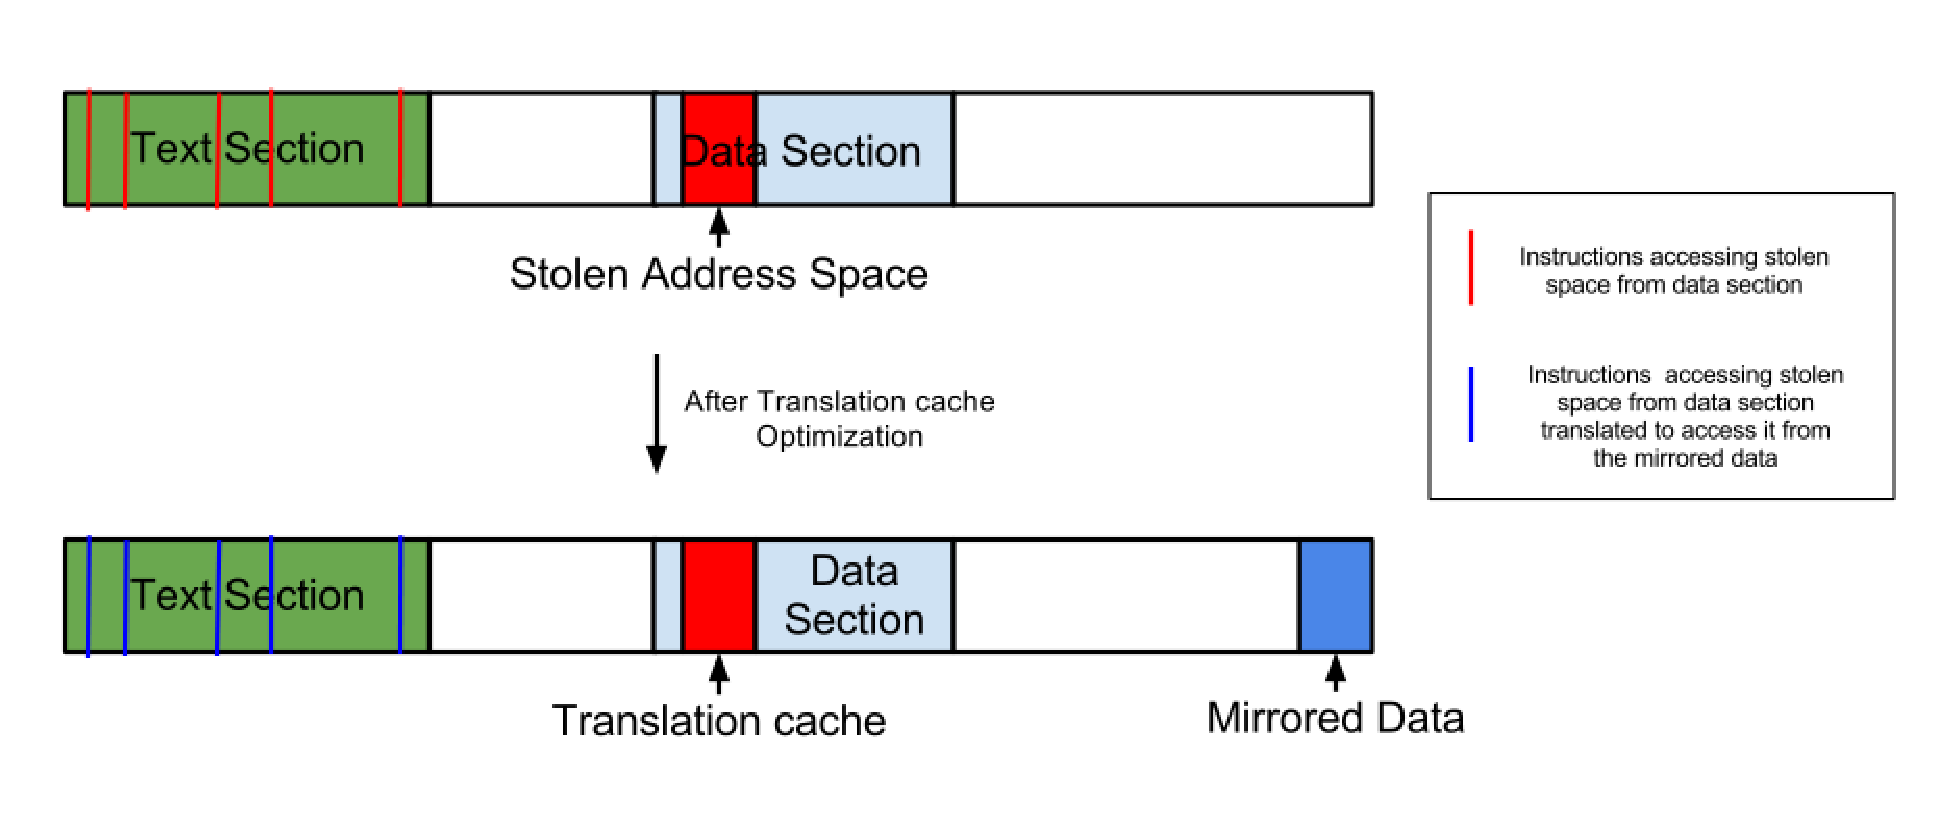
\includegraphics[scale=0.4]{tcache_opt.eps}
\caption{\label{fig:translation_cache_stealing}Translation cache {\tt Setup} and its {\tt Optimization} shown inside guest kernel address space}
\end{figure}

\begin{table*}
\centering
      \begin{tabular}{|l| p{3.1cm} |p{3.1cm}|p{3.1cm}|} \hline
        Benchmark\verb, ,& {\tt Guest allocated Tcache} \verb, ,& {\tt Stolen} \verb, ,& {\tt Stolen \& optimized} \verb, , \\ \hline

     & \multicolumn{3}{c|}{Running Time in $sec$}\\ \cline {2-4}
Linux boot	&	12.24	&	14.39	&	12.39	\\
Echo Spawn	&	7.26	&	8.90	&	6.85	\\
Find	&	0.67	&	1.67	&	0.83	\\
Lame	&	0.51	&	0.50	&	0.50	\\
\hline
      \end{tabular}
\caption{\label{tab:tcache}Measuring the overhead and performance when translation cache is allocated by guest, in comparison to a when translation cache is being stored in stolen space but without any optimizations and when translation cache is being stored in stolen space with data mirroring optimizations.}
\end{table*}







